\section{Ejercicio N02 - Reservas de viaje} 

En este esquema de E / R, un cliente (que es de cierto tipo) reserva un viaje en una agencia de viajes. La agencia de viajes
trabaja para un determinado operador turístico. El viaje va a un destino determinado que pertenece a un país determinado.
La dimensión de tiempo consiste en mes, trimestre y año.

	\begin{center}
	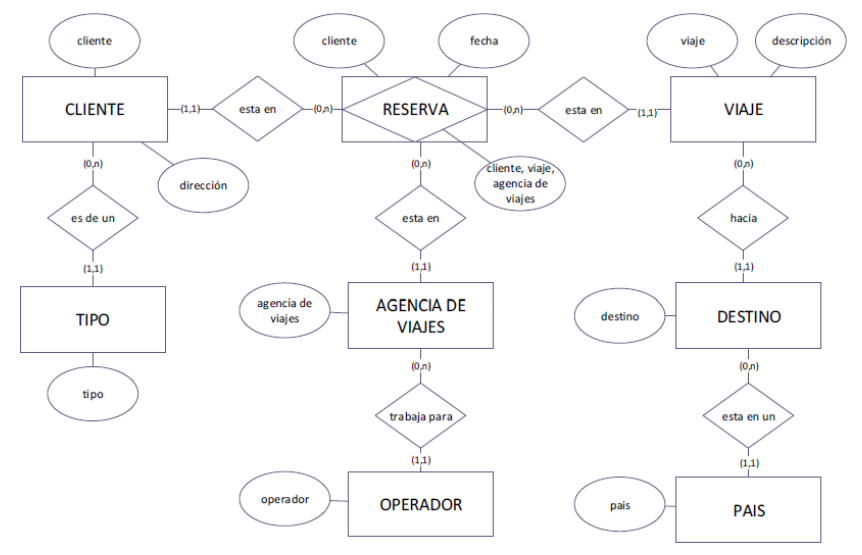
\includegraphics[width=17cm]{./Imagenes/ejercicio2}
	\end{center}	

Por favor identifique el hecho de interés y construya el Modelo Dimensional y su respectivo esquema físico.
\\

\begin{itemize}
    \item \textbf{Modelo Dimensional}
\\
El diseñador de software ERWIN permite que se pueda crear y modificar diagramas con facilidad, mejorando la calidad de los diseños de software. El Modelo Dimensional es el resultado directo de la llegada del diseño de flujo de datos y análisis estructural.

	\begin{center}
	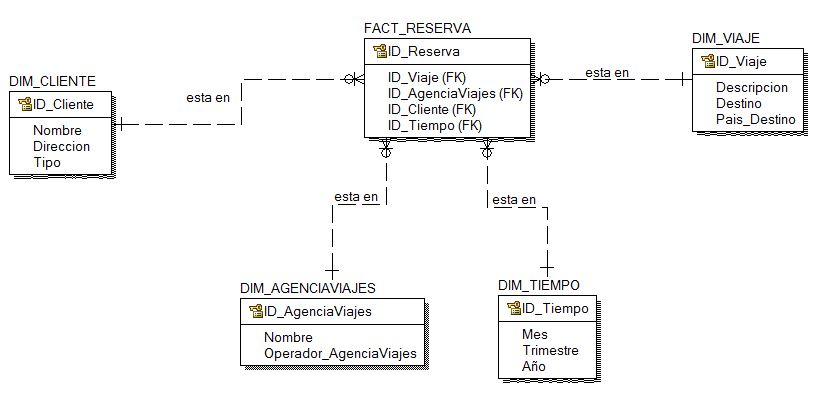
\includegraphics[width=17cm]{./Imagenes/Ejercicio2Logico}
	\end{center}	

    \item \textbf{Modelo Fisico}

Es posible crear y modificar bases de datos de forma visual a través de los diagramas de bases de Datos. Estos diagramas fisicos proporcionan una visión gráfica de las tablas en la base de datos incluyendo sus columnas, el modelo E/R y el diagrama fisico de estructura de datos en SQL Server.

	\begin{center}
	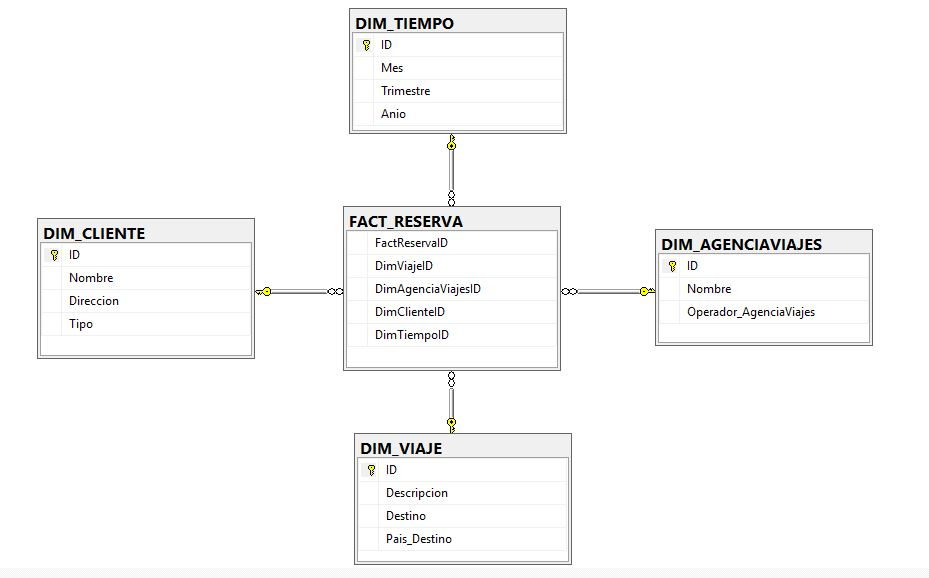
\includegraphics[width=17cm]{./Imagenes/Ejercicio2Fisico}
	\end{center}	

    \item \textbf{Código del Modelo Fisico}

	\begin{center}
	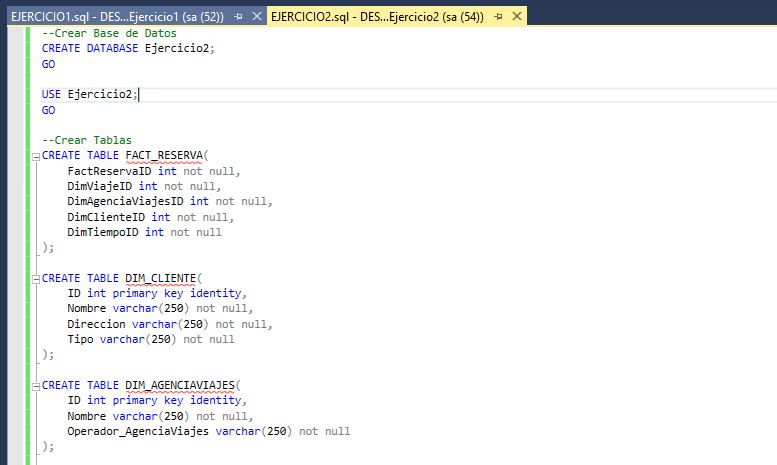
\includegraphics[width=17cm]{./Imagenes/Ejercicio2Fisico1}
	\end{center}	

	\begin{center}
	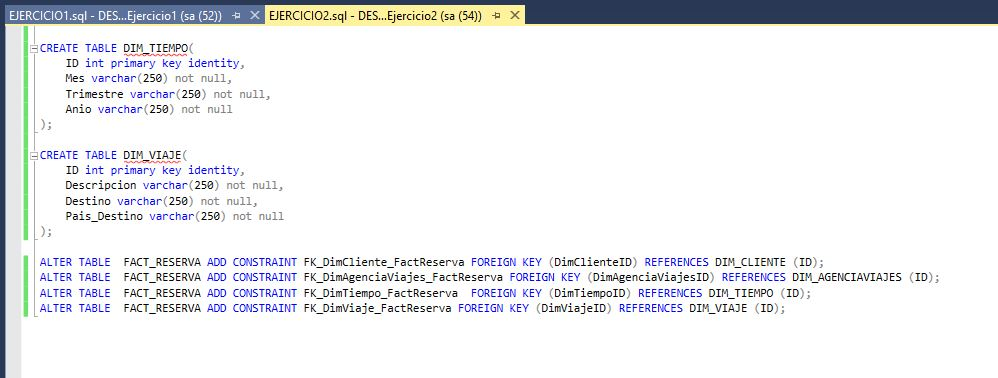
\includegraphics[width=17cm]{./Imagenes/Ejercicio2Fisico2}
	\end{center}	
\end{itemize}